% Ablation Study Results Visualization
% Generated for CCSE-CS paper
\begin{figure}[t]
\centering
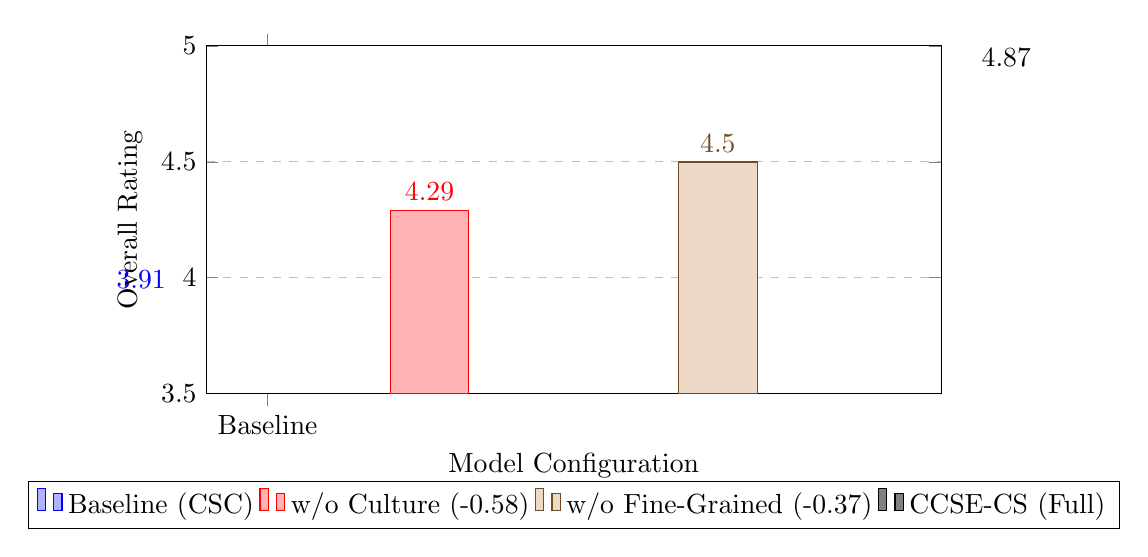
\begin{tikzpicture}
\begin{axis}[
    ybar,
    width=0.9\textwidth,
    height=6cm,
    symbolic x coords={Baseline, w/o Culture, w/o Fine-Grained, Full Model},
    xtick=data,
    nodes near coords,
    nodes near coords align={vertical},
    ymin=3.5, ymax=5.0,
    ylabel={Overall Rating},
    xlabel={Model Configuration},
    legend style={at={(0.5,-0.25)}, anchor=north, legend columns=-1},
    ymajorgrids=true,
    grid style=dashed,
    bar width=1cm,
]

% Baseline (CSC)
\addplot coordinates {(Baseline, 3.912)};

% w/o Culture (remove 4-dimensional cultural framework)
\addplot coordinates {(w/o Culture, 4.289)};

% w/o Fine-Grained (use coarse-grained strategies)
\addplot coordinates {(w/o Fine-Grained, 4.499)};

% Full Model (CCSE-CS)
\addplot coordinates {(Full Model, 4.869)};

\legend{Baseline (CSC), w/o Culture (-0.58), w/o Fine-Grained (-0.37), CCSE-CS (Full)}

\end{axis}

\end{tikzpicture}
\caption{Ablation study results showing the contribution of each component. Removing the four-dimensional cultural framework results in -0.58 performance drop, while using coarse-grained strategies results in -0.37 drop, validating both contributions.}
\label{fig:ablation_results}
\end{figure}
